\documentclass{article}
\usepackage{amsmath}
\usepackage{tikz}
\usepackage{pgfplots}
\usepackage{graphicx}

\begin{document}
Naloge sem reševal samostojno. Reševal sem v C++ z Eigen knjižnico za linearno algebro, 3D ploti za poročilo prve naloge pa so v pythonu (zato ker uporabljam linux in knjižnice za izrisovanje pogosto ne delujejo na Windowsu brez veliko dela, tako da bi vi imeli težave pri poganjanju kode), ampak je samo klic surface\_plot() matrike, ki sem jo v C++ shranil v datoteko. Podobno sem python uporabil za pretvorbo .mat datoteke za 4. nalogo v .mtx format, ki ga lahko bere Eigen - že pretvorjene matrike prilagam. Slike so malo grdo razporejene po poročilu, ker imajo veliko belega prostora - če piše "Figure \(n\)" spadajo k prvi nalogi.

\section{Naloga 1}
    Naj bo \(U(x,y) = U_{x,y}\) matrika
    \begin{align*}
        \Delta u(x,y) = U_{xx} + U_{yy}\\
        h\cdot U_x = U(x) - U(x+1)\\
        h^2\cdot U_{xx} = U(x-1, y) - 2U(x,y) + U(x+1,y)\\
        h^2\cdot U_{yy} = U(x, y-1) - 2U(x,y) + U(x, y+1)
    \end{align*}
    Če to damo skupaj, dobimo
    \begin{align*}
        \Delta U(x,y) + k(x,y)U(x,y) = 1\\
        h^2 = U(x-1,y)+U(x+1,y)+U(x,y-1)+U(x,y+1) + (h^2\cdot k(x,y)- 4) U(x,y)
    \end{align*}
    Vemo, da je \(U(i,j)=0\) na \(\partial [-1,1]^2\) oziroma \(\{0,n\}\times [0,n]\) in obratno. V matriki za relacije računamo ostale vrednosti.
    
    Problem preuredimo v enačbo \(Ax=b\) kjer je \(x\) \(n\cdot n\) vektor, ki predstavlja rešitev \(u(i,j) = x_{n*i+j}\). Relacije od zgoraj sestavimo v matriko; stran \(b\) je kar \(h^2\) v vseh komponentah. Diagonalni elementi so ponavadi \(4\), razen ko upoštevamo kaznovalni parameter \(k\).

    \begin{figure}[h!]
        \centering
        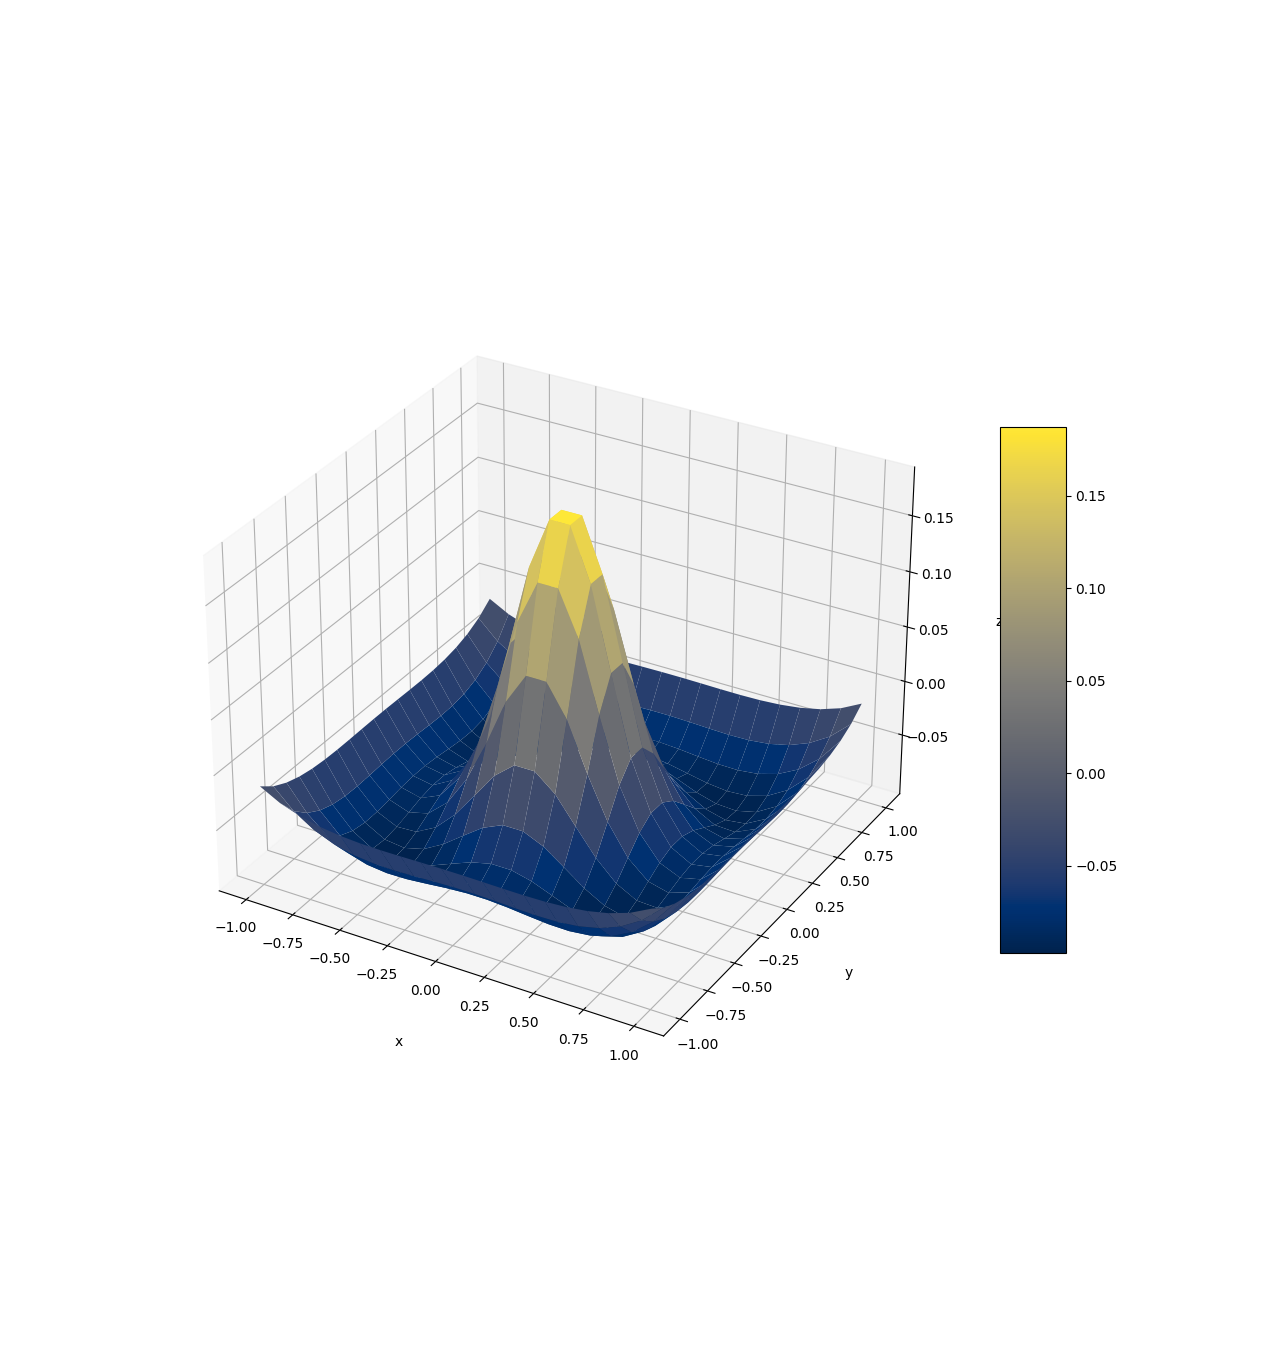
\includegraphics[width=0.9\textwidth]{nal1_n20_k50.png}
        \caption{n 20, k 50}
    \end{figure}

    \begin{figure}[h!]
        \centering
        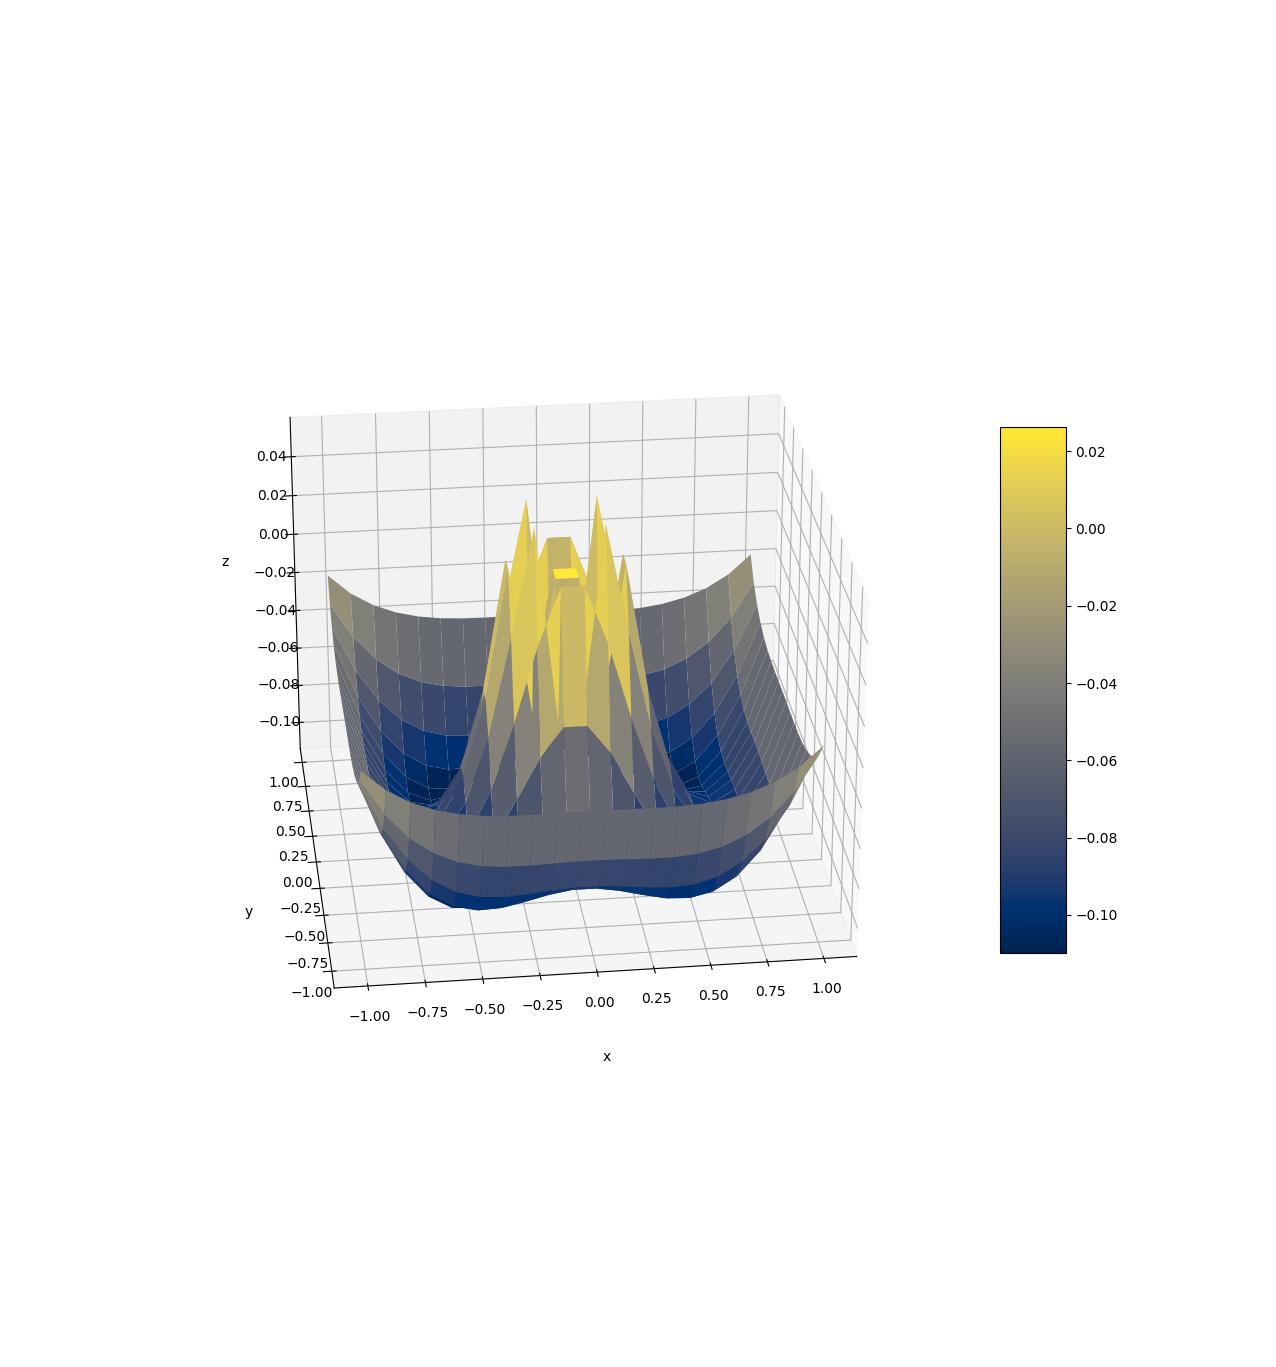
\includegraphics[width=0.9\textwidth]{nal1_n20_k500.png}
        \caption{n 20, k 500}
    \end{figure}

    \begin{figure}[h!]
        \centering
        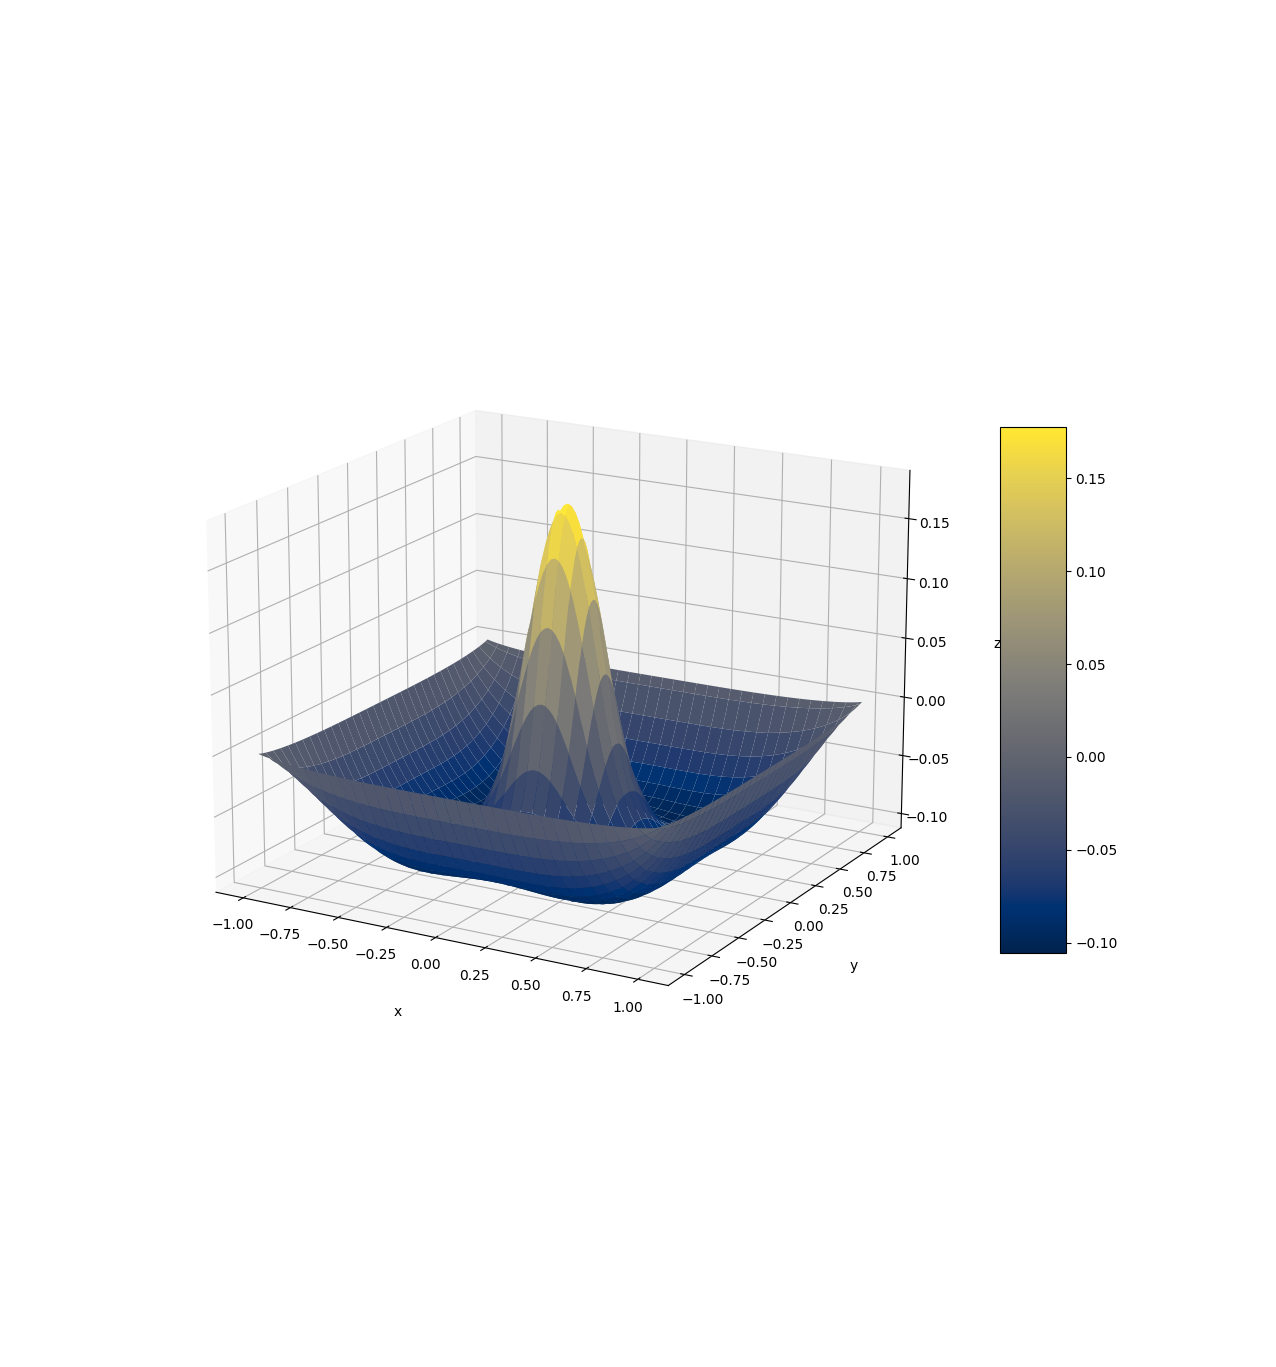
\includegraphics[width=0.9\textwidth]{nal1_n101_k100.png}
        \caption{n 101, k 100}
    \end{figure}

    \begin{figure}[h]
        \centering
        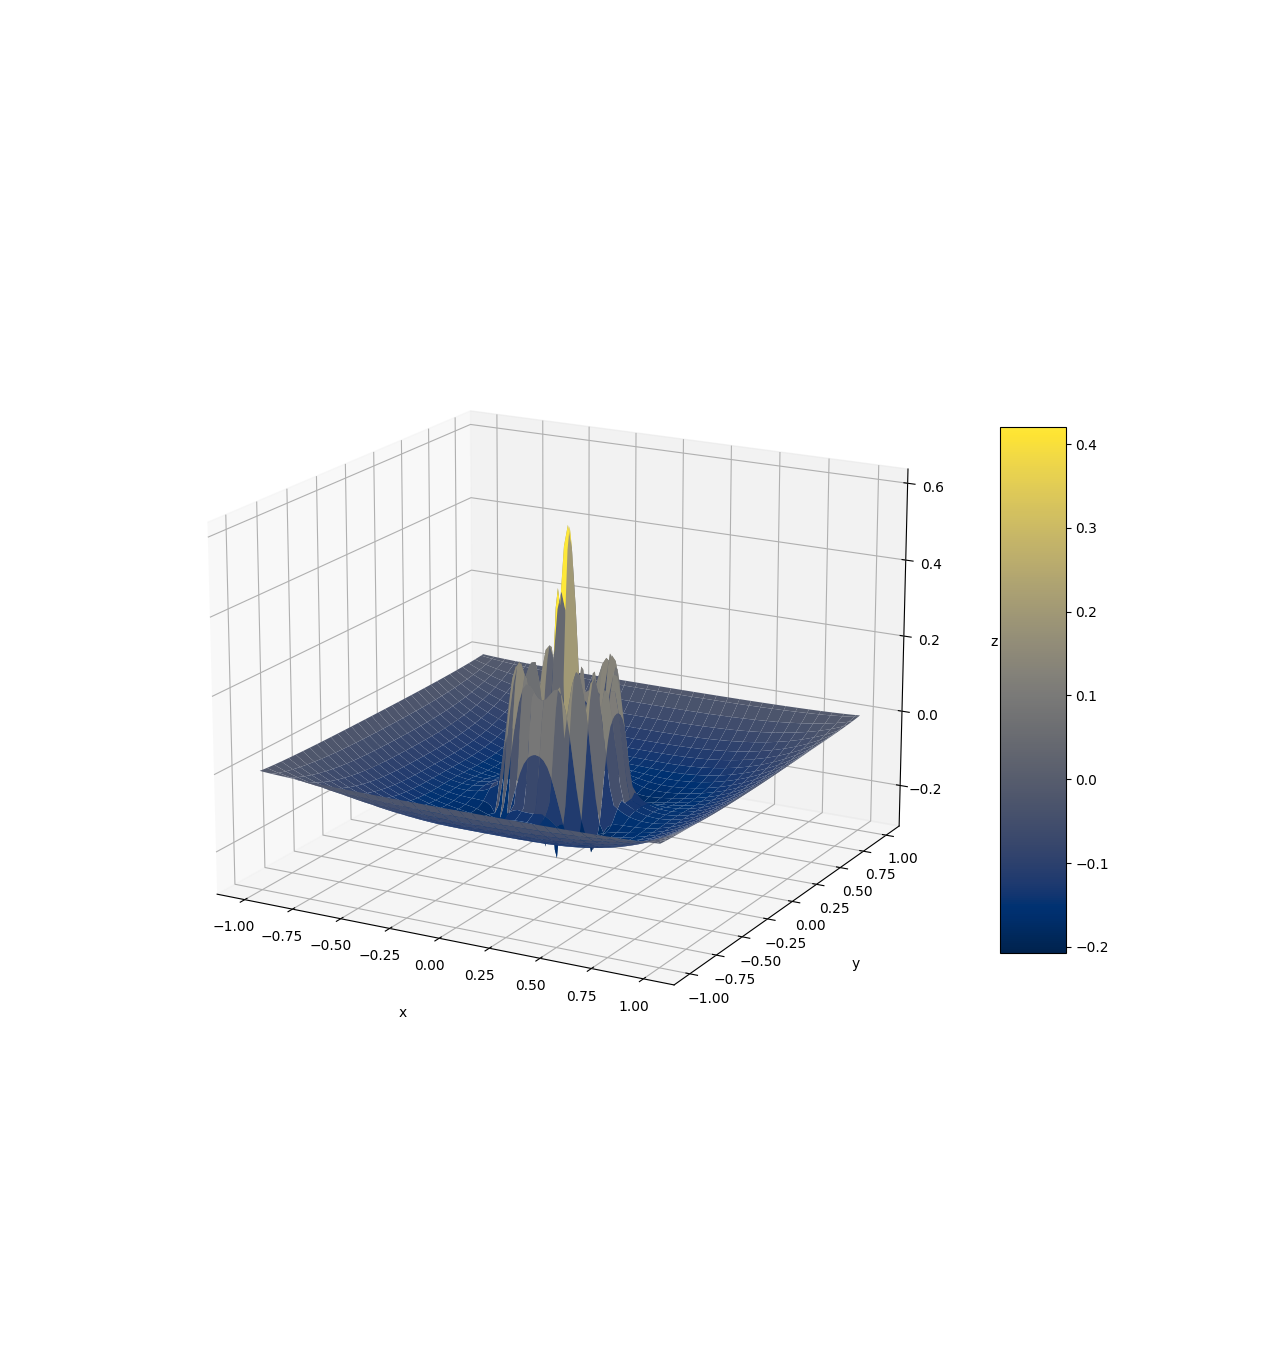
\includegraphics[width=0.9\textwidth]{nal1_n101_k1000.png}
        \caption{n 101, k 1000}
    \end{figure}

    \begin{figure}[h]
        \centering
        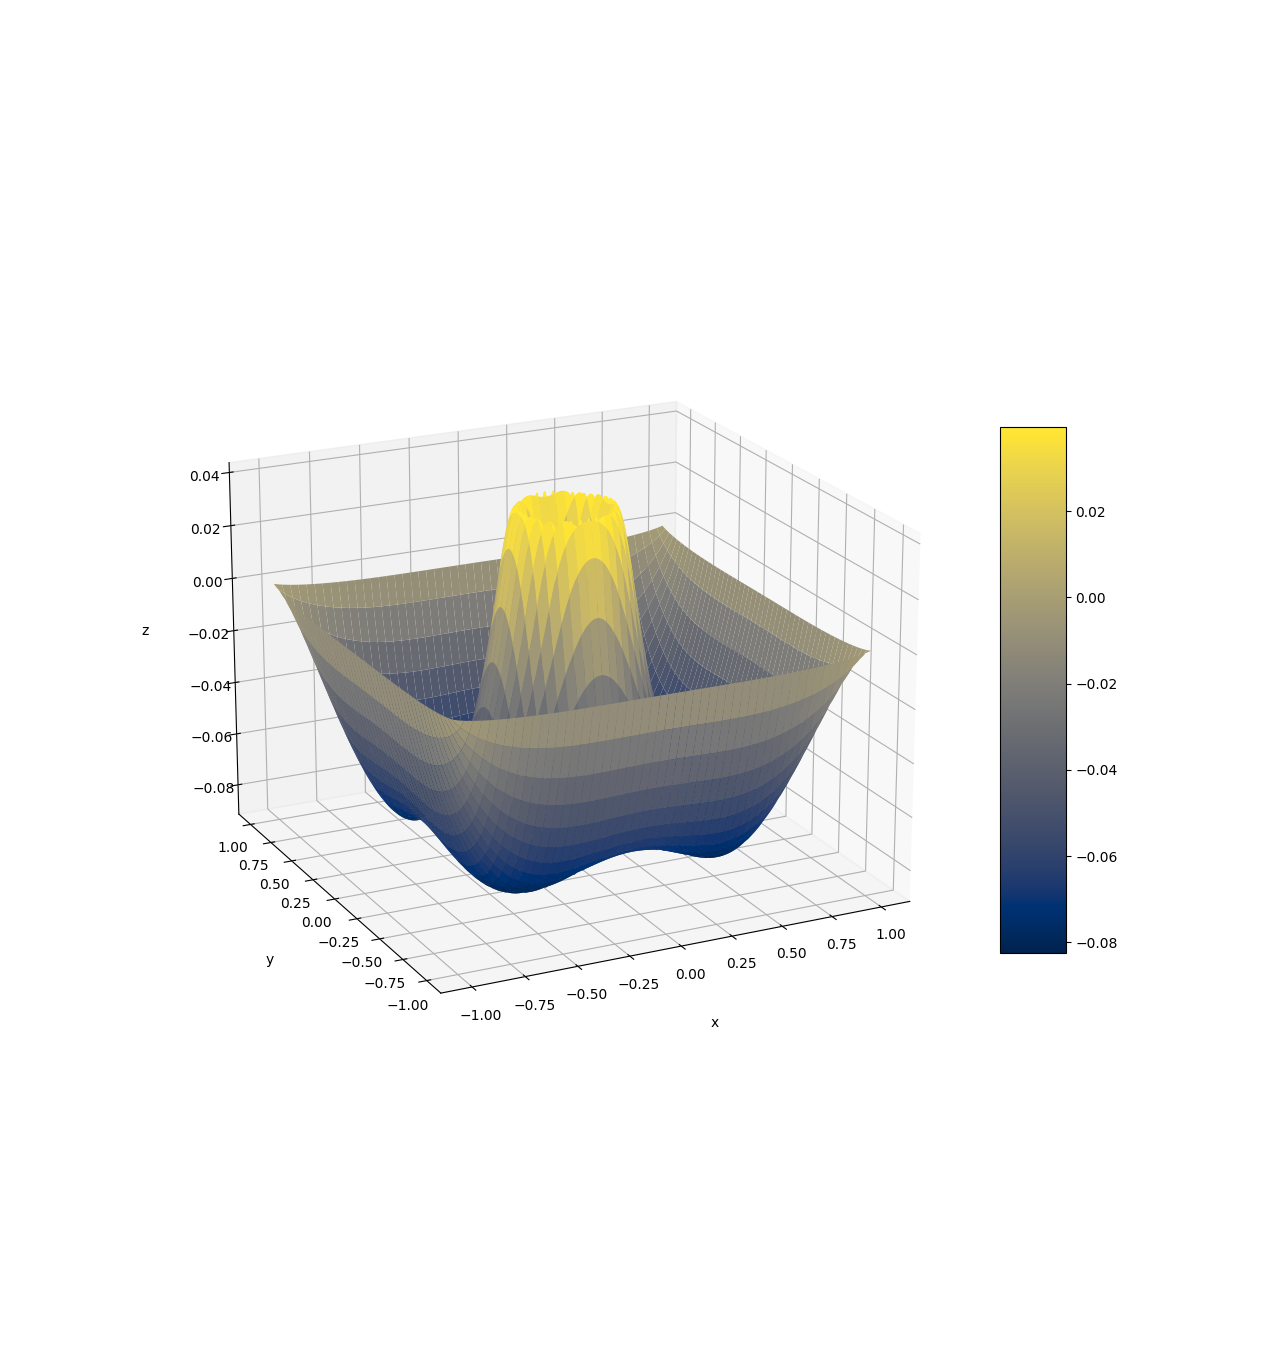
\includegraphics[width=0.9\textwidth]{nal1_n200_k300.png}
        \caption{n 200, k 300}
    \end{figure}

    \begin{figure}[h]
        \centering
        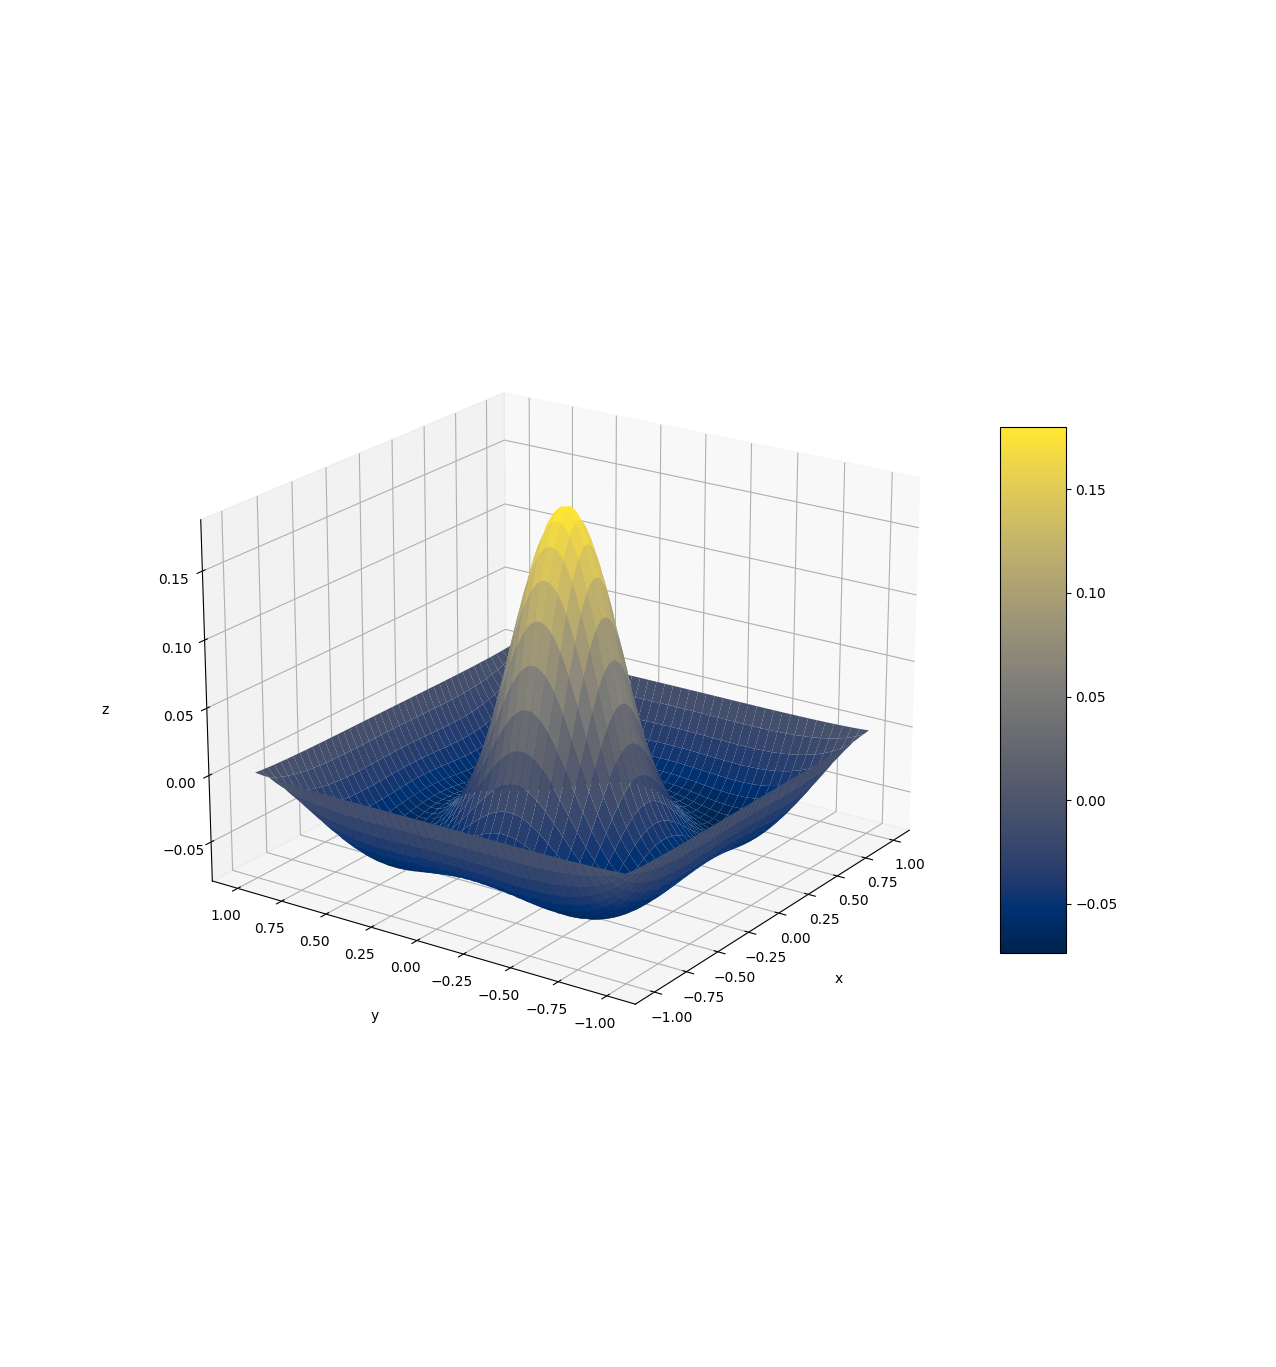
\includegraphics[width=0.9\textwidth]{nal1_n301_k50.png}
        \caption{n 301, k 50}
    \end{figure}

    \begin{figure}[h]
        \centering
        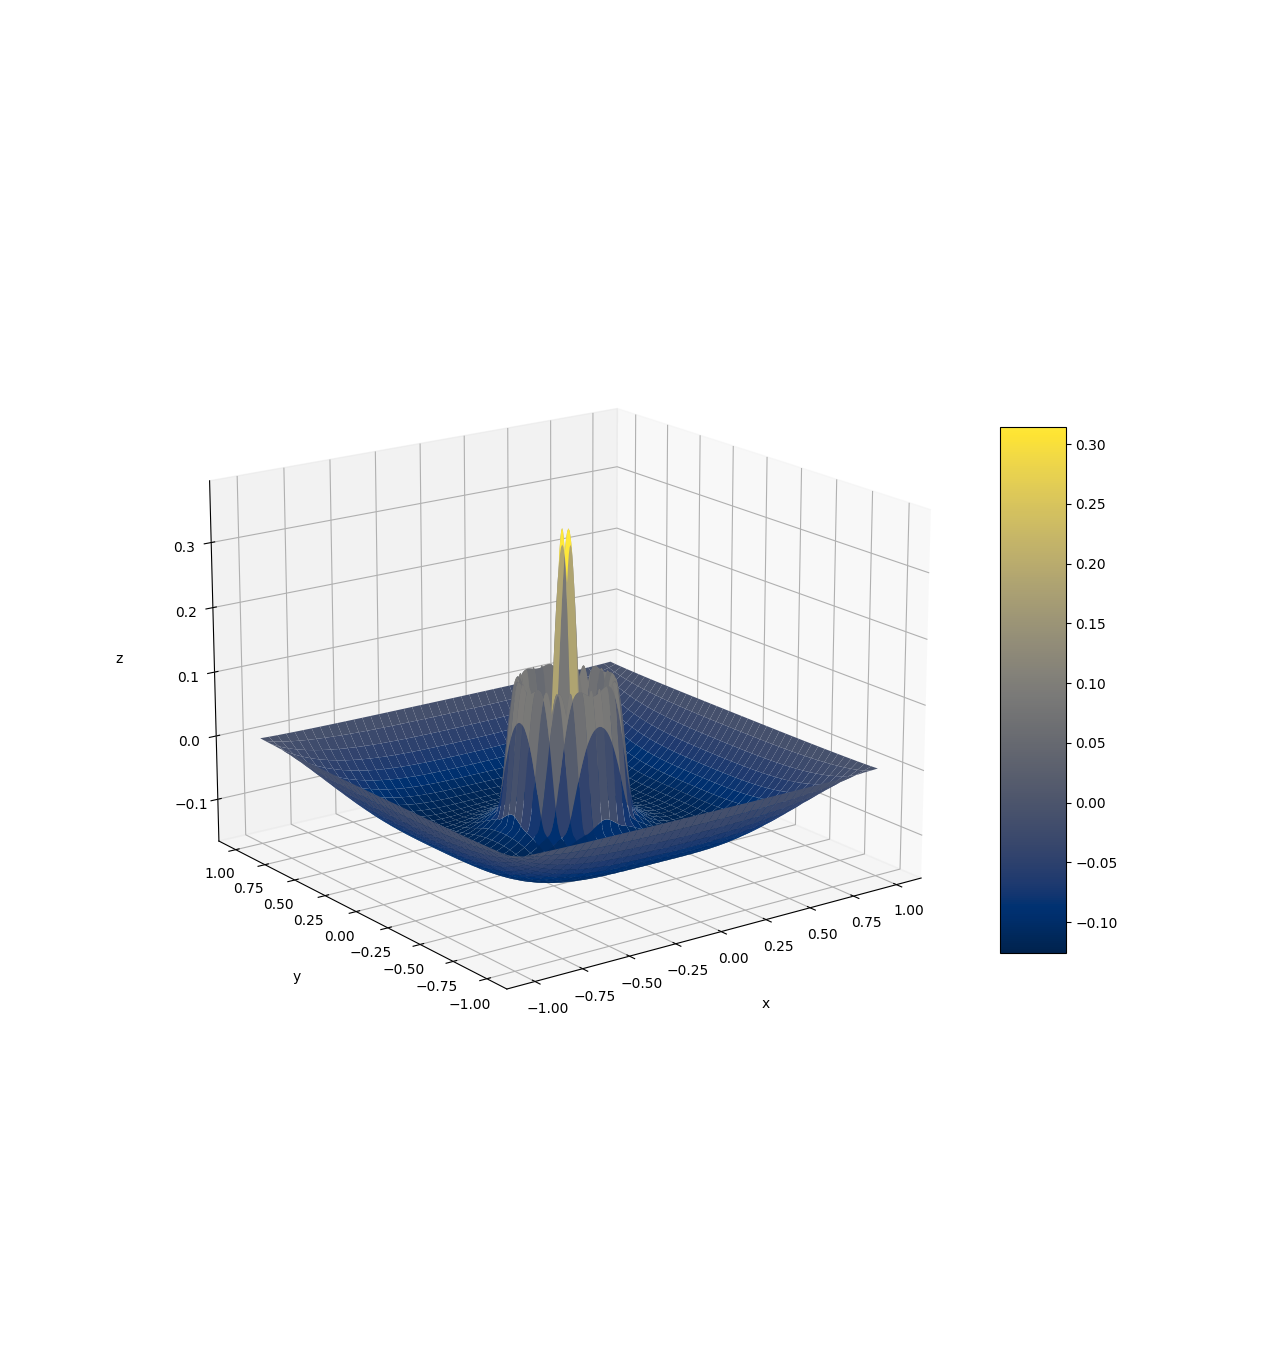
\includegraphics[width=0.9\textwidth]{nal1_n301_k1000.png}
        \caption{n 301, k 1000}
    \end{figure}

    \begin{figure}[h]
        \centering
        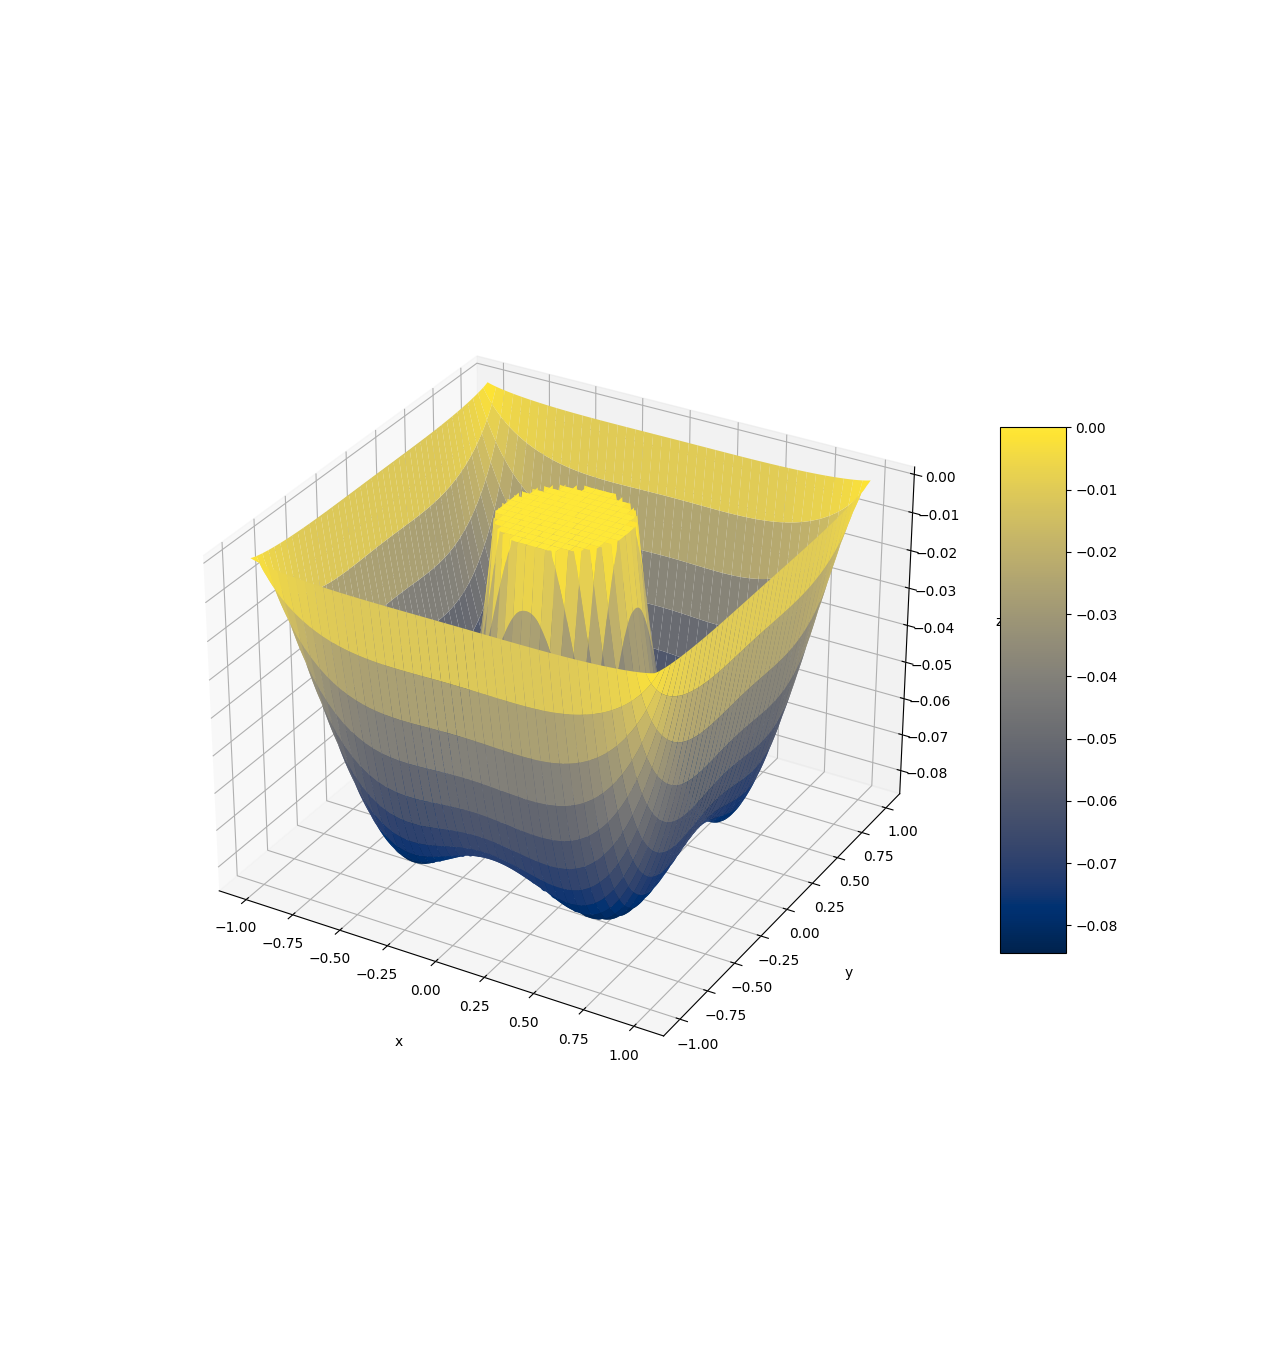
\includegraphics[width=0.9\textwidth]{nal1_n301_k1e6.png}
        \caption{n 301, k 1 000 000}
    \end{figure}

    \begin{figure}[h]
        \centering
        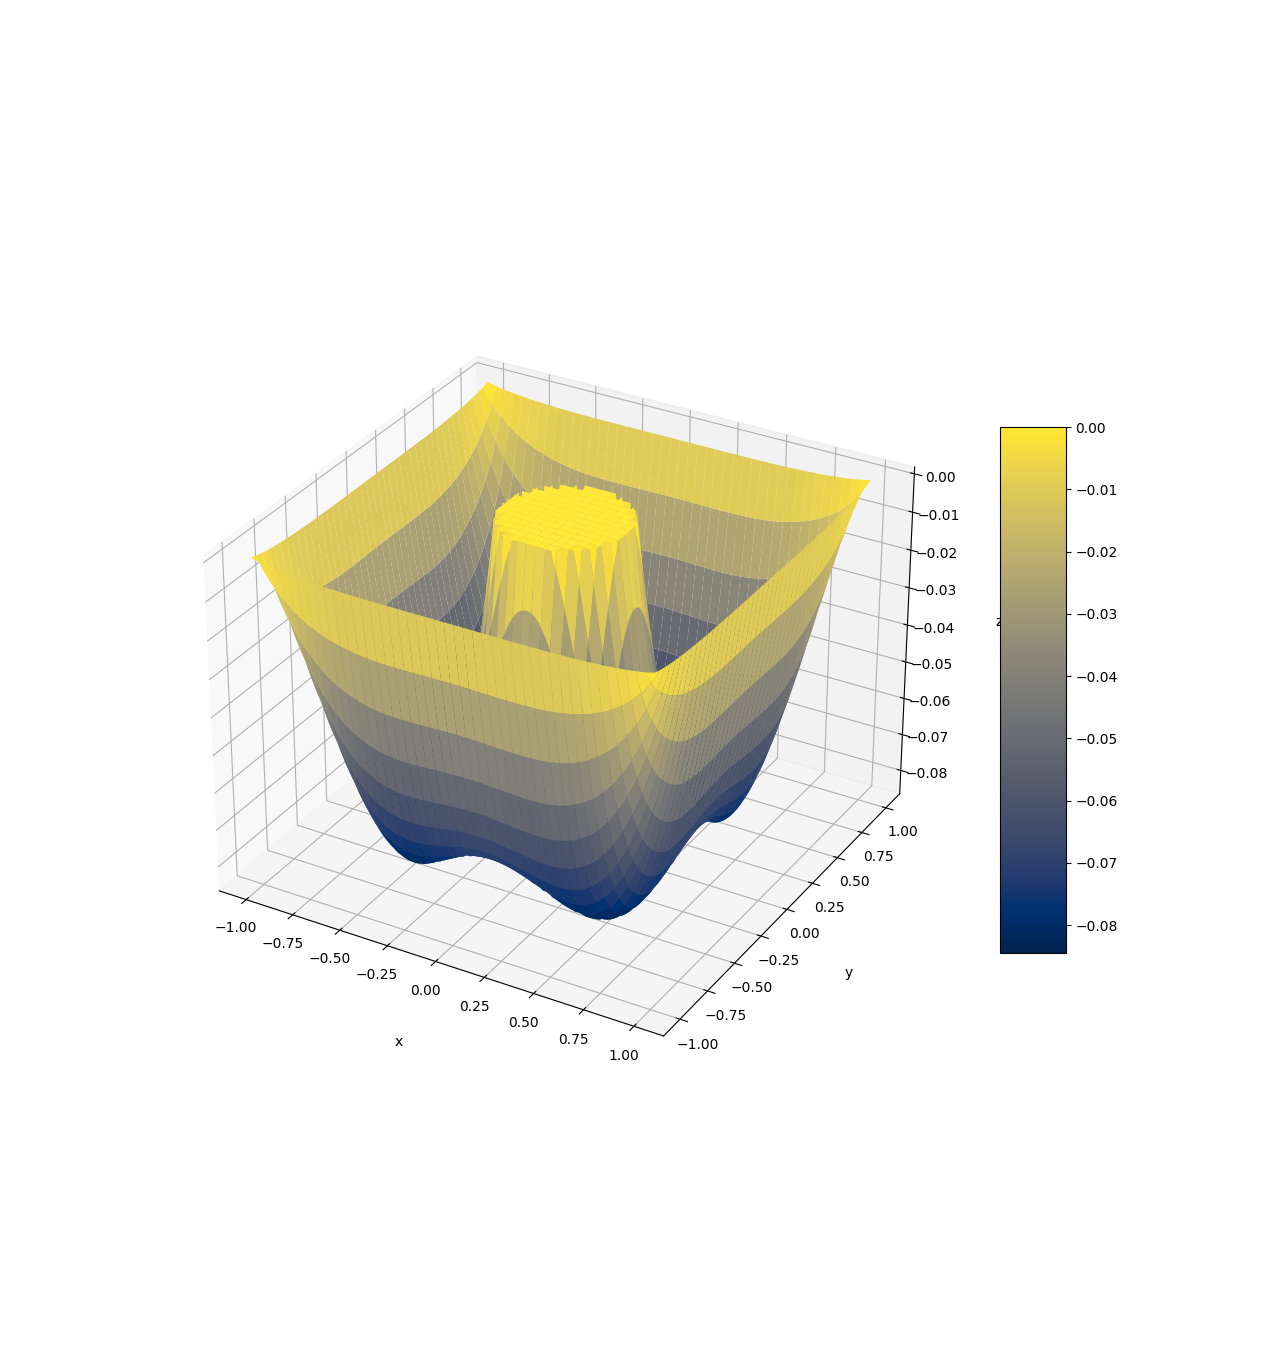
\includegraphics[width=0.9\textwidth]{nal1_n301_k1e9.png}
        \caption{n 301, k 1 000 000 000}
    \end{figure}

    \begin{figure}[h]
        \centering
        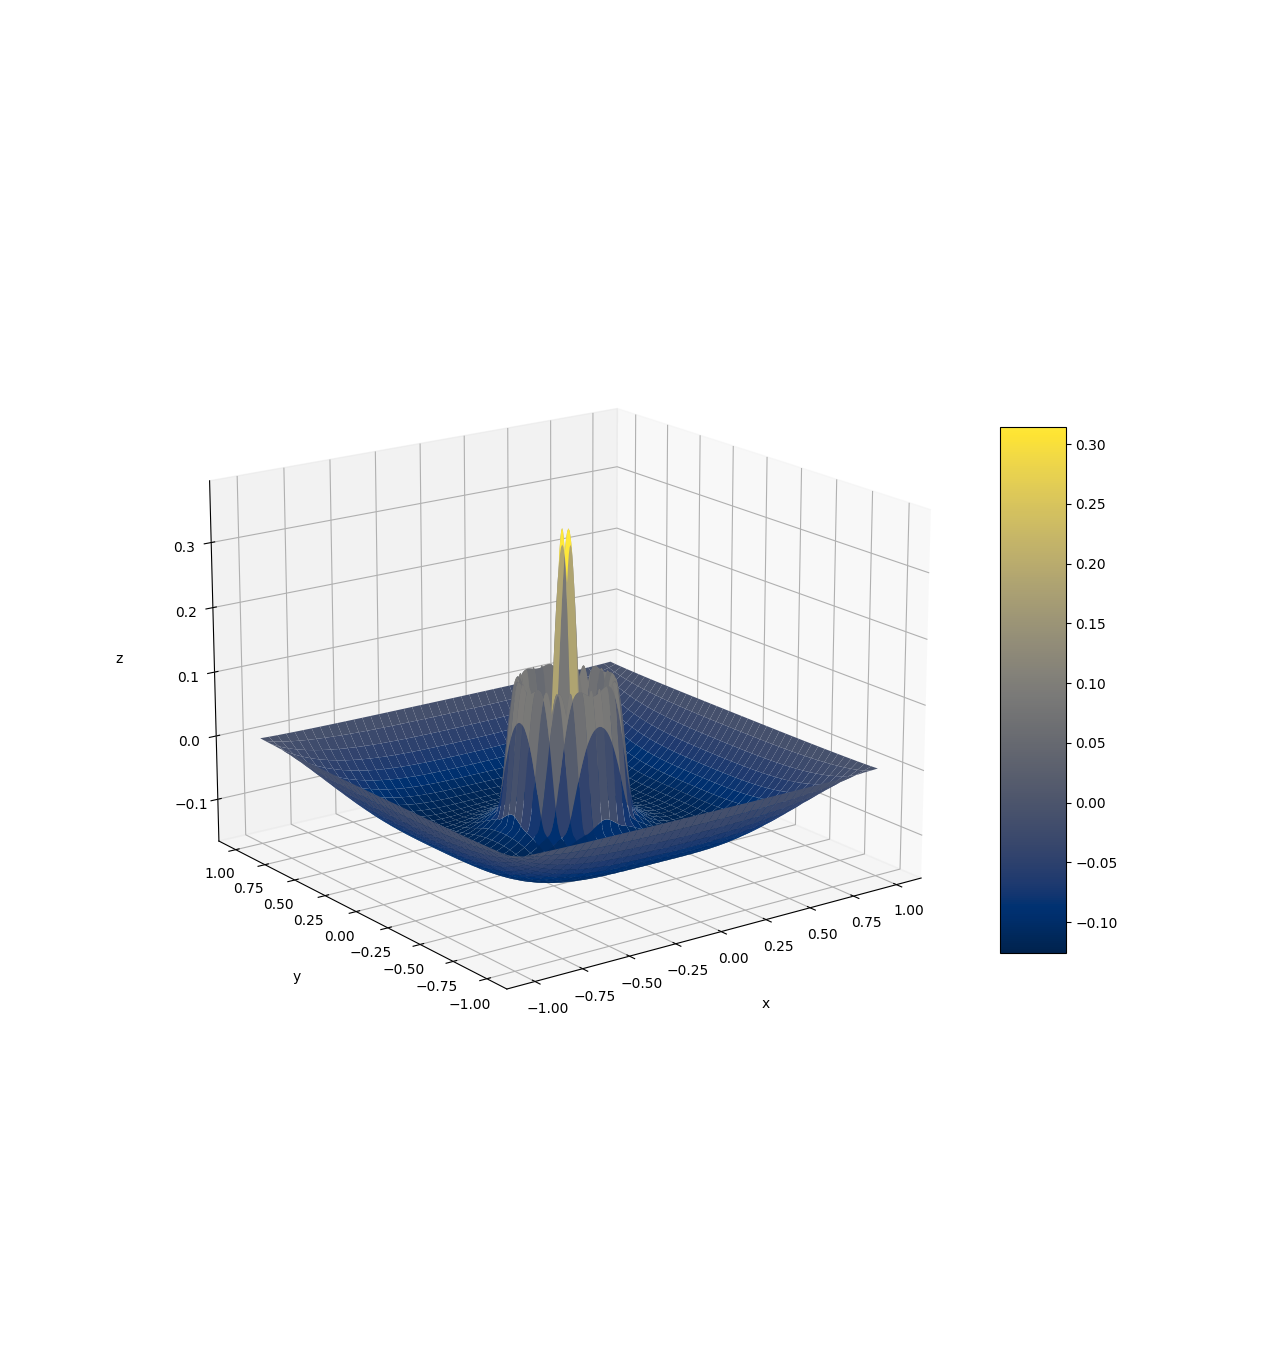
\includegraphics[width=0.9\textwidth]{nal1_n301_k1000.png}
        \caption{n 301, k 1000}
    \end{figure}

    \begin{figure}[h]
        \centering
        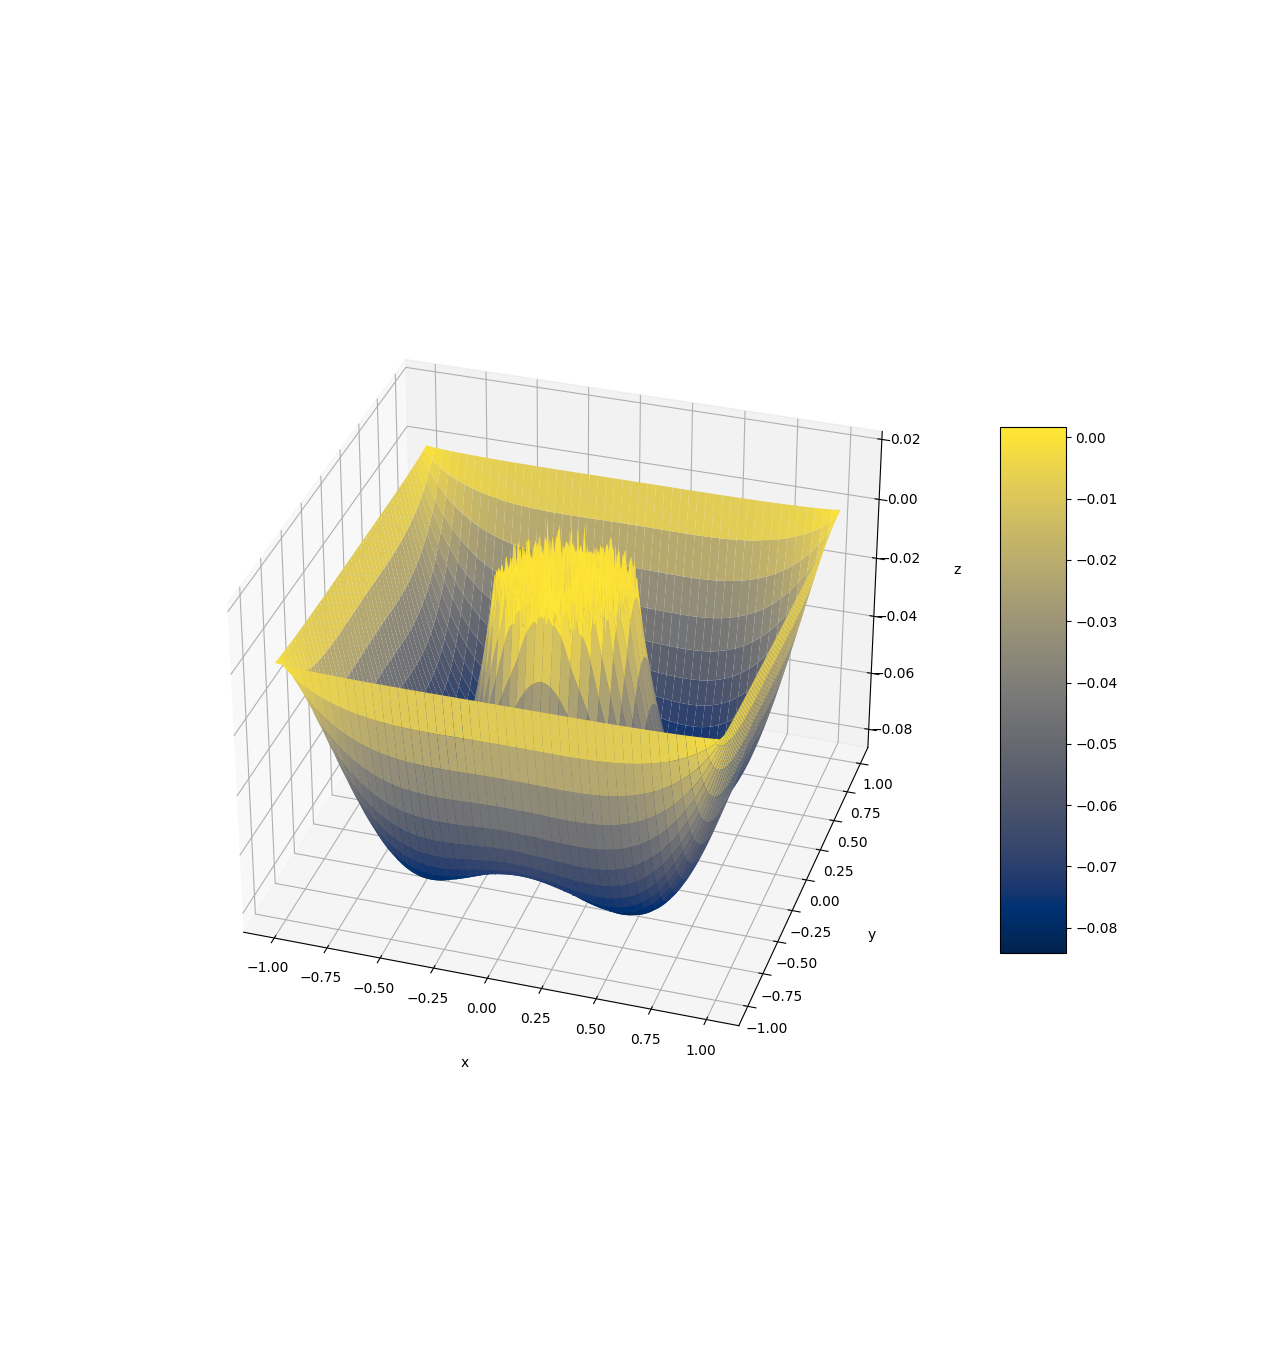
\includegraphics[width=0.9\textwidth]{nal1_n600_k100000.png}
        \caption{n 600, k 100000}
    \end{figure}

    Višji kot je \(n\), boljšo rešitev dobimo, saj vzorčimo bolj drobne delce (in teoretična izpeljava deluje le, ko gre \(n\to \infty\)). Do numeričnih težav ne pride za smiselne vrednosti \(n\) (na primer pod nekaj tisoč), če bi pa pretiravali bi pa lahko prišlo do težav.

    Kaznovalni parameter poskrbi, da so vrednosti na krogu približno enake 0, saj dobimo enačbo oblike \(k\cdot u = 1- \Delta \), kar je približno \(h^2 k u = O(u)\). Torej, da poskrbimo, da je \(u\) majhen, more biti \(h^2k>>0\). To lahko naredimo tako, da (neoptimalno) uporabimo \(k\approx n^3\) ali pa \(k\approx C\cdot n^2\).

    Višji kot je \(k\) boljši približek dobimo (lahko uporabimo tudi \(k=\infty\), vendar je teoretična analiza potem nerodna). Če je ta dovolj velik (kot v prejšnjih ocenah) je matrika šibko diagonalno dominantna (in nerazcepna) in lahko uporabimo iterativno metodo. Za dan problem dobro deluje Jacobijeva metoda, ki konvergira. 

    \begin{figure}[h]
        \centering
        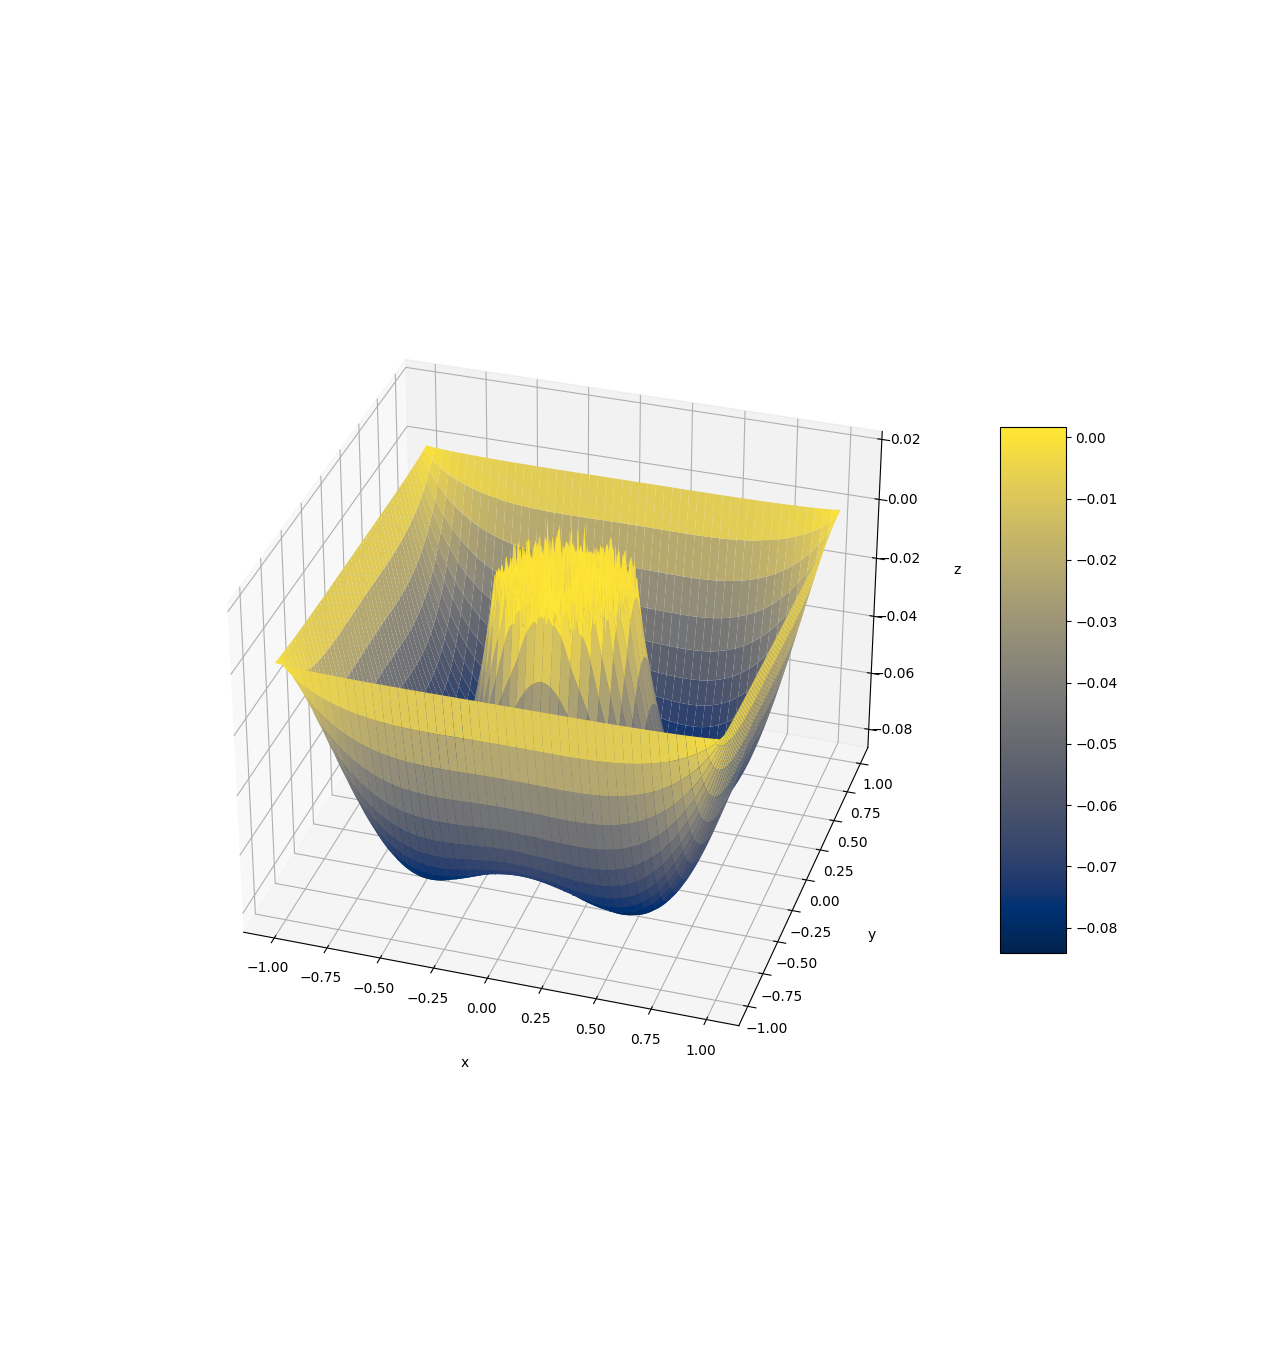
\includegraphics[width=0.9\textwidth]{nal1_n600_k100000.png}
        \caption{n 301, k 1e6, Jacobi s 3000 iteracij}
    \end{figure}

    
    \section{Naloga 2}
    Nedokončana. V datoteki spišem D-Lanczos algoritem (ki deluje) z LU razcepom in ga uporabim, da popravim na QR razcep. 

    Če pišemo podobno izpeljavo kot za LU D-Lanczos, vidimo
    \begin{align*}
        x_k = x_0 + V_kT_k^{-1}\lVert r_0\rVert e_1\\
        x_0 + V_k R_k^{-1} Q_k^\top \lVert r_0 \rVert e_1\\
        P_k R_k= V_k\\
        z_k = Q_k^\top \lVert r_0 \rVert e_1
    \end{align*}
    Če napišemo \(Q_k\) kot \(G_1^\top \cdots G_k^\top\) (kjer so \(G_i\) Givensove rotacije) dobimo zadnjo vrstico
    \begin{align*}
        Q_k^\top = G_k \cdots G_1
    \end{align*}
    Torej je \(\zeta_k = s\cdot \zeta_{k-1}'\). Vendar pa se v zaradi Givensove rotacije spremeni tudi \(\zeta_{k-1} = c\cdot \zeta_{k-1}'\).

    Podobno analizo delamo pri \(R_k\). Vemo, da je pri QR razcepu od tridiagonalne matrike \(R\) zgornja trikotna matrika z le tremi neničelnimi naddiagonalami, torej lahko element \(p_k\) napišemo kot \(p_k = (v_k - \lambda_0 p_{k-2} - \lambda_1 p_{k-1})/\lambda_2\), kjer je \(\lambda_2\) diagonalni element matrike v zadnjem stolpcu, \(\lambda_1\) naddiagonalni in \(\lambda_2\) nad naddiagonalnim. Tukaj je spet potrebno popravljati koeficient še v naslednji iteraciji, saj ga naslednja givensova rotacija spremeni, vendar lahko to poskrbimo brez da hranimo dodatni vektor (hranimo le koeficiente in givensove rotacije, kar je poceni). Potrebno je torej hraniti \(p_k\), \(p_{k-1}\), \(p_{k-2}\), \(A\), \(x\), \(b\) in konstantno mnogo številskih parametrov.

    Moja implementirana metoda ne deluje, ker sem se jo lotil pisati nespametno ter potem raje reševal druge naloge, osnutek je pa končan v kodi (do permutacije vrstic natančno, saj bi bilo treba pravilno upoštevati rotacije).


    \section{Naloga 3}
    Vse metode uporabljamo z toleranco 1e-6 in maksimalnim številom korakov 500. Izhod programa je priložen v datoteki \verb|output.txt| (saj se sicer izvaja precej dolgo časa). namesto nekaterih Matlabovih metod sem uporabil ostale Eigen iterativne metode (idrs, idrstabl, idrstab, bicgstabl).
    
    Najlepša matrika je gridgena. Na njej delujejo vse metode, saj je simetrična in SPD. Uporabimo lahko tudi dobro predpogovjevanje, saj je cholesky razgradljiva. Še posebej uporabne so metode idrstabl, bicgstabl in gmres s predpogojevanjem choleskega. Zaradi izjemno hitre konvergence (v le 15 iteracijah) parameter ponovnega zagona nima velikega vpliva. Predpogojevanje pomaga mnogim metodam: metodi minres, idrs, idrstabl in bistab delajo najboljebolje z diagonalnim predpogojevanjem; gmres, cg pa s predpogojevanjem choleskega. Idrstabl z diagonalnim predpogojevanjem deluje hitreje kot metoda SparseLU.

    Slabše se obnaša c-63. Je sicer simetrična, ni pa pozitivno definitna ali Cholesky razgradljiva. Metode s privzetimi nastavitvami so počasne. Najbolje delata idrstabl in bicgstabl, sprejemljivo pa kovnergira tudi gmres brez ponovnega zagona, kjer potrebuje 254 iteracij z 64 restart in 103 iteracij brez ponovnega zagona. Za manjše vrednosti restarta ne konvergira znotraj 500 iteracij. Če dodamo diagonalno predpogojevanje se konvergenca veliko pospeši. Zelo dobro delajo vse metode (razen minres zaradi tehničnih razlogov). Če uporabimo predpogojevanja lahko tudi rešimo hitreje kot SparseLU z vsemi metodami.

    RFDevice ima za \(b\) matriko z devetimi stolpci. Stolpca \(0\) in \(4\) sta slabša od ostalih, za njiju ne deluje dobro nobena iterativna metoda. Pri ostalih stolpcih gmres prez predpogojevanja pride do rešitve v petih korakih. Sprejemljive metode so tudi bicgstab in idrs in idrstabl. Predpogojevanja le poslabšajo rezultate.




    \section{Naloga 4}
    Da določimo optimalen \(\alpha\) poženemo algoritem za različne \(\alpha\) s privzeto toleranco (okoli 1e-15). Spremljamo, koliko korakov je bilo potrebnih za konvergenco. Nato preverimo odstopanje rešitve od neregularizirane rešitve.


    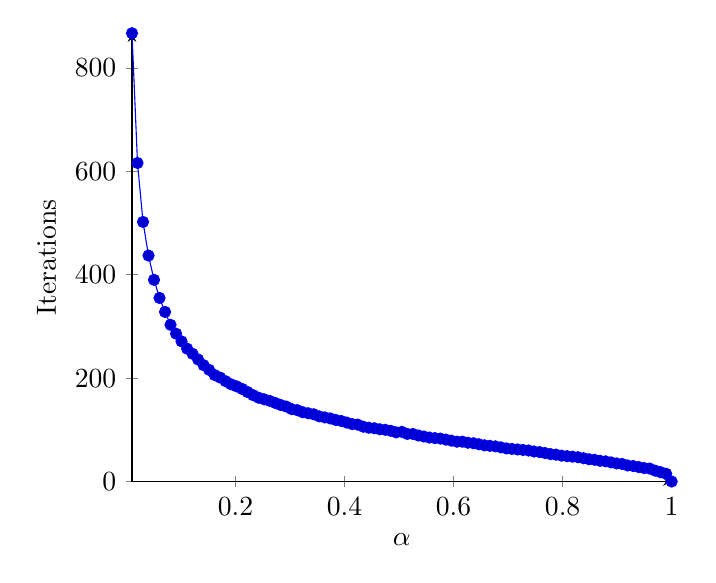
\begin{tikzpicture}
        \centering
        \begin{axis}[
            axis lines = left,
            xlabel = {\(\alpha\)},
            ylabel = {Iterations}
        ]
        \addplot coordinates {
                (0.010101, 867)
                (0.020202, 616)
                (0.030303, 502)
                (0.040404, 437)
                (0.050505, 390)
                (0.0606061, 355)
                (0.0707071, 328)
                (0.0808081, 303)
                (0.0909091, 286)
                (0.10101, 271)
                (0.111111, 257)
                (0.121212, 247)
                (0.131313, 236)
                (0.141414, 225)
                (0.151515, 216)
                (0.161616, 206)
                (0.171717, 201)
                (0.181818, 194)
                (0.191919, 188)
                (0.20202, 184)
                (0.212121, 179)
                (0.222222, 173)
                (0.232323, 167)
                (0.242424, 162)
                (0.252525, 159)
                (0.262626, 156)
                (0.272727, 152)
                (0.282828, 148)
                (0.292929, 145)
                (0.30303, 140)
                (0.313131, 138)
                (0.323232, 134)
                (0.333333, 132)
                (0.343434, 130)
                (0.353535, 126)
                (0.363636, 124)
                (0.373737, 122)
                (0.383838, 119)
                (0.393939, 117)
                (0.40404, 114)
                (0.414141, 111)
                (0.424242, 110)
                (0.434343, 106)
                (0.444444, 104)
                (0.454545, 103)
                (0.464646, 101)
                (0.474747, 100)
                (0.484848, 98)
                (0.494949, 95)
                (0.50505, 96)
                (0.515152, 92)
                (0.525253, 92)
                (0.535354, 89)
                (0.545455, 87)
                (0.555556, 85)
                (0.565657, 84)
                (0.575758, 83)
                (0.585859, 81)
                (0.59596, 79)
                (0.606061, 77)
                (0.616162, 77)
                (0.626263, 75)
                (0.636364, 74)
                (0.646465, 72)
                (0.656566, 70)
                (0.666667, 69)
                (0.676768, 68)
                (0.686869, 66)
                (0.69697, 64)
                (0.707071, 63)
                (0.717172, 62)
                (0.727273, 61)
                (0.737374, 60)
                (0.747475, 58)
                (0.757576, 57)
                (0.767677, 55)
                (0.777778, 53)
                (0.787879, 52)
                (0.79798, 50)
                (0.808081, 49)
                (0.818182, 48)
                (0.828283, 47)
                (0.838384, 45)
                (0.848485, 43)
                (0.858586, 42)
                (0.868687, 40)
                (0.878788, 39)
                (0.888889, 37)
                (0.89899, 35)
                (0.909091, 34)
                (0.919192, 31)
                (0.929293, 30)
                (0.939394, 28)
                (0.949495, 26)
                (0.959596, 25)
                (0.969697, 21)
                (0.979798, 18)
                (0.989899, 15)
                (1, 0)
            };
        \end{axis}
    \end{tikzpicture}

    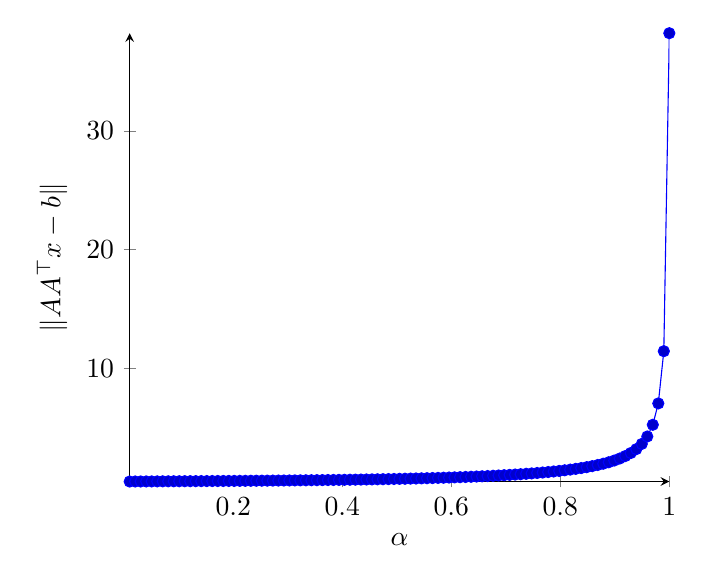
\begin{tikzpicture}
        \centering
        \begin{axis}[
            axis lines = left,
            xlabel = {\(\alpha\)},
            ylabel = {\(\lVert AA^\top x - b\rVert\)}
        ]
        \addplot coordinates {
            (0.010101, 0.458222)
(0.020202, 0.460376)
(0.030303, 0.462818)
(0.040404, 0.465419)
(0.050505, 0.468106)
(0.0606061, 0.470839)
(0.0707071, 0.473596)
(0.0808081, 0.476368)
(0.0909091, 0.479151)
(0.10101, 0.481945)
(0.111111, 0.484754)
(0.121212, 0.487581)
(0.131313, 0.490431)
(0.141414, 0.493311)
(0.151515, 0.496226)
(0.161616, 0.499183)
(0.171717, 0.502188)
(0.181818, 0.505247)
(0.191919, 0.508369)
(0.20202, 0.511559)
(0.212121, 0.514824)
(0.222222, 0.518173)
(0.232323, 0.521612)
(0.242424, 0.525148)
(0.252525, 0.528789)
(0.262626, 0.532544)
(0.272727, 0.536419)
(0.282828, 0.540424)
(0.292929, 0.544566)
(0.30303, 0.548854)
(0.313131, 0.553297)
(0.323232, 0.557905)
(0.333333, 0.562688)
(0.343434, 0.567654)
(0.353535, 0.572815)
(0.363636, 0.578181)
(0.373737, 0.583763)
(0.383838, 0.589574)
(0.393939, 0.595625)
(0.40404, 0.601929)
(0.414141, 0.6085)
(0.424242, 0.615351)
(0.434343, 0.622498)
(0.444444, 0.629956)
(0.454545, 0.637741)
(0.464646, 0.645871)
(0.474747, 0.654363)
(0.484848, 0.663238)
(0.494949, 0.672515)
(0.50505, 0.682216)
(0.515152, 0.692364)
(0.525253, 0.702984)
(0.535354, 0.714102)
(0.545455, 0.725746)
(0.555556, 0.737945)
(0.565657, 0.750733)
(0.575758, 0.764144)
(0.585859, 0.778214)
(0.59596, 0.792984)
(0.606061, 0.808499)
(0.616162, 0.824805)
(0.626263, 0.841953)
(0.636364, 0.860001)
(0.646465, 0.879011)
(0.656566, 0.899049)
(0.666667, 0.920191)
(0.676768, 0.942519)
(0.686869, 0.966126)
(0.69697, 0.991113)
(0.707071, 1.0176)
(0.717172, 1.0457)
(0.727273, 1.07558)
(0.737374, 1.10739)
(0.747475, 1.14132)
(0.757576, 1.17759)
(0.767677, 1.21645)
(0.777778, 1.25818)
(0.787879, 1.30314)
(0.79798, 1.35172)
(0.808081, 1.40439)
(0.818182, 1.46175)
(0.828283, 1.52448)
(0.838384, 1.59345)
(0.848485, 1.66974)
(0.858586, 1.75473)
(0.868687, 1.85016)
(0.878788, 1.95836)
(0.888889, 2.08245)
(0.89899, 2.22673)
(0.909091, 2.39733)
(0.919192, 2.60328)
(0.929293, 2.85855)
(0.939394, 3.18593)
(0.949495, 3.6253)
(0.959596, 4.25349)
(0.969697, 5.23951)
(0.979798, 7.04002)
(0.989899, 11.4415)
(1, 38.2373)
            };
        \end{axis}
    \end{tikzpicture}

    Iz grafa razberemo, da je za vrednost \(\alpha=0.6\) rešitev zelo blizu dejanske rešitve, število iteracij pa zadovoljivo nizko. Računamo matriko \(X^\top A^{-1} X\). Zaradi učinkovitosti v spomin shranimo le en stolpec končnega rezultata na enkrat in ga shranimo v datoteko (column major format, tako da izgleda, kot da shranimo transponiranko).
    
    Računanja stolpca \(i\) se lotimo tako, da preslikamo \(e_i\) z \(X\), kar nam da \(x_i\). Nato rešimo sistem \(Ay = x_i\) z metodo konjugiranih gradientov. Rešitev \(y\) preslikamo z \(X\), da dobimo \(i\)-ti stolpec končne matrike.
\end{document}